%--------------------------------------------------------%
%	TITLE
%--------------------------------------------------------%

\chapter[Anthropogenic Basin Closure and Groundwater Salinization (ABCSAL)]{Anthropogenic Basin Closure and Groundwater Salinization (ABCSAL).\footnote[1]{This chapter has been submitted to \textit{Journal of Hydrology}: Pauloo, R. A., Fogg, G. E., Guo, Z., \& Harter, T. ``Anthropogenic Basin Closure and Groundwater Salinization (ABCSAL)''. (Preprint 10.1002/essoar.10502733.1)}}

%--------------------------------------------------------%
%	ABSTRACT
%--------------------------------------------------------%
\section{Abstract}

\noindent Global food systems rely on irrigated agriculture, and most of these systems in turn depend on fresh sources of groundwater. In this study, we demonstrate that groundwater development, even without overdraft, can transform a fresh, open basin into an evaporation dominated, closed-basin system, such that most of the groundwater, rather than exiting via stream baseflow and lateral subsurface flow, exits predominantly by evapotranspiration from irrigated lands. In these newly closed hydrologic basins, just as in other closed basins, groundwater salinization is inevitable because dissolved solids cannot escape, and the basin is effectively converted into a salt sink. We first provide a conceptual model of this process, called ``\textbf{A}nthropogenic \textbf{B}asin \textbf{C}losure and groundwater \textbf{SAL}inization'' (ABCSAL). We examine the temporal dynamics of ABCSAL using the Tulare Lake Basin, California, as a case study for a large irrigated agricultural region with Mediterranean climate, overlying an unconsolidated sedimentary aquifer system. Even with modern water management practices that arrest historic overdraft, results indicate that shallow aquifers (36 $m$ deep) exceed maximum contaminant levels for total dissolved solids on decadal timescales. Intermediate (132 $m$) and deep aquifers (187 $m$), essential for drinking water and irrigated crops, are impacted within two to three centuries. Hence, ABCSAL resulting from groundwater development constitutes a largely unrecognized constraint on groundwater sustainable yield on similar timescales to aquifer depletion in the Tulare Lake Basin, and poses a serious challenge to groundwater quality sustainability, even when water levels are stable. Results suggest that agriculturally intensive groundwater basins worldwide may be susceptible to ABCSAL.

%--------------------------------------------------------%
% Introduction
%--------------------------------------------------------%
\section{Introduction}  


Groundwater from major aquifer systems supplies 43\% of the world's irrigation water \citep{Siebert2010}. As a result of excessive groundwater development and land use change, groundwater quantity and quality in these agriculturally intensive groundwater basins has been significantly impacted. Numerous global and regional studies document aquifer depletion related to agricultural withdrawal \citep{Brush2013, Doll2012, Famiglietti2014, Faunted.2009, Gleeson2012, Russo2017, Scanlon2012, Siebert2010, Vorosmarty2014, Wada2014}. Anthropogenic contaminants to groundwater include nitrates, which originate from agricultural fertilizers \citep{Burow2008}, pesticides \citep{Burow2008, Burow1998}, and animal farming \citep{Harter2012}. Groundwater pumping may even mobilize naturally-occurring contaminants such as arsenic \citep{winkel2011arsenic, smith2018overpumping} and uranium \citep{Jurgens2008, Jurgens2010}.

Another class of groundwater contaminants are total dissolved solids (TDS), also referred to as salts or salinity. TDS are sourced both naturally (e.g., produced by rock-water interactions) and anthropogenically (e.g., imported by surface water for irrigation). 
Elevated TDS is an indicator of human impact on freshwater systems \citep{Ayers1985, Kaushal2014}, and reduces agricultural productivity \citep{Lopez-Berenguer2009, Munns2002, Pessarakli2011}, which has prompted states to set agricultural irrigation water quality goals, (e.g., 450 mg/L in California) \citep{swrcb2019b}. For drinking water, the United States Environmental Protection Agency and the state of California recommend a secondary maximum contaminant level of 500 mg/L TDS \citep{swrcb2019a, swrcb2019b}. Water high in TDS may exhibit discoloration, unpleasant odor and taste, and may be unsuitable for human consumption or irrigation \citep{Hem1985}. Fresh water is defined as containing TDS less than 1,000 mg/L, brackish water ranges from 1,000 to 10,000 mg/L, and saline water ranges from 10,000 to 100,000 mg/L \citep{Fetter2001}. 

Groundwater salinization is widely studied \citep{Greene2016soil} in terms of (1) seawater intrusion \citep{bear1999seawater, Werner2013}, (2) naturally-occurring salinization in closed surface-water basins (i.e., endorheic basins and playas) \citep{Eugster1978, Hardie1970}, (3) high water tables causing groundwater evaporation and soil salinization via capillary rise \citep{Datta2002, barrett2003interaction, chaudhuri2014, hillel1992out}, and (4) soil salinization due to irrigation \citep{hanson1999agricultural, bernstein1973leaching, hillel2000salinity}. This study describes a fifth type of groundwater salinization that remains largely unexplored: salinization of an entire groundwater basin created by historically excessive pumping, then sustained by the inability of a closed groundwater system to discharge salts. Henceforth, we refer to this fifth type as ``\textbf{A}nthropogenic \textbf{B}asin \textbf{C}losure and groundwater \textbf{SAL}inization'' (ABCSAL). 

This fifth type of salinization, ABCSAL, is related to naturally-occurring closed basin salinization (case (2) above), but has significantly different phenomenology. It is therefore useful to first consider the difference between an open, fresh hydrologic basin, and a naturally closed, saline basin. 

An open, fresh groundwater basin has sufficient natural outlets for TDS, such as baseflow to streams and lateral subsurface flow across basin boundaries, which maintains a balance between salinity that is naturally generated within the basin (i.e., mineral dissolution) and salinity that is exported out of the basin. Basins containing fresh groundwater exist only because they have outlets for both the circulating groundwater and the dissolved salts therein, originating from intrabasin rocks and sediments \citep{domenico1998physical}. 

In contrast, closed hydrologic basins -- common in arid to semiarid regions worldwide -- naturally form when (a) outflow by surface water or groundwater flows is absent or small, and (b) evaporation is the dominant mechanism by which water exits the basin \citep{Hardie1970, Eugster1978, Jones1978}. Because TDS concentrations in precipitation are low (around $10^1$ $mg/L$), most TDS originates from rock-water reactions in surface runoff and in the subsurface. Salts may accumulate at the evaporative boundaries of the basin: at or immediately below the surface where discharging groundwater evaporates or at the bottom of a surface depression in terminal and sometimes ephemeral lakes that collect runoff, baseflow, and spring outflow \citep{Wooding1997, richter1986geochemistry}. Examples of naturally closed hydrologic basins with saline features at or near the land surface are found worldwide: playas and salt flats such as those in the Great Basin (USA) and Salar de Uyuni (Bolivia); saline lakes like the Great Salt Lake (USA) and the Dead Sea (Middle east); in extremely arid deserts such as the Arabian and Atacama; and in the unsaturated subsurface of semi-arid regions with insufficient precipitation to recharge groundwater \citep{Scanlon1997, kreitler1993geochemical}. 

In this paper, we argue that sufficient groundwater development can lower groundwater levels in an open to semi-open and relatively fresh basin, thus converting it into a closed basin, which then salinates in a distinctly different manner from those described in (1) - (4). First, moderate to large amounts of groundwater development may result in sufficient reduction of groundwater levels that reduce or eliminate natural baseflow to streams \citep{Russo2017, Barlow2015, Hunt1999} and reverse existing groundwater gradients at subsurface outflow boundaries (Figure \ref{fig:conceptual_model_gw_sal}A). Progressively greater closed basin conditions diminish and eventually entirely eliminate natural TDS export from the groundwater basin (Figure \ref{fig:conceptual_model_gw_sal}B). Furthermore, if the basin is irrigated, crop evapotranspiration becomes the dominant water outflow from the basin, leaving behind salts that are returned to the groundwater basin via irrigation return flows and recharge from precipitation. Across the globe, water level stabilization in such overdrafted basins is sometimes achieved by importing additional surface water. However, water imports can add significant salt to the basin. Moreover, even when balancing the water budget with imported water, this does not stop the ABCSAL process if groundwater does not have exits (e.g., baseflow to streams or lateral subsurface outflow), and if water continues to leave the basin predominantly through evapotranspiration, which leaves behind salts. Although these latter two conditions are similar to those in a naturally closed basin (2) \citep{Hardie1970, Jones1978}, vertical groundwater fluxes under ABCSAL are in the opposite direction from natural basin salinization and thus, the location of salinization is different. In a naturally closed basin, salinization occurs at the land surface due to upward groundwater discharge. Under ABCSAL, pumping and recharge from irrigation lead to a net downward flux, then mobilize salts left behind by irrigated crops downward into the production zone of the groundwater basin, before they are recycled by pumping wells to the land surface and the process repeats.

\begin{figure}[ht]
	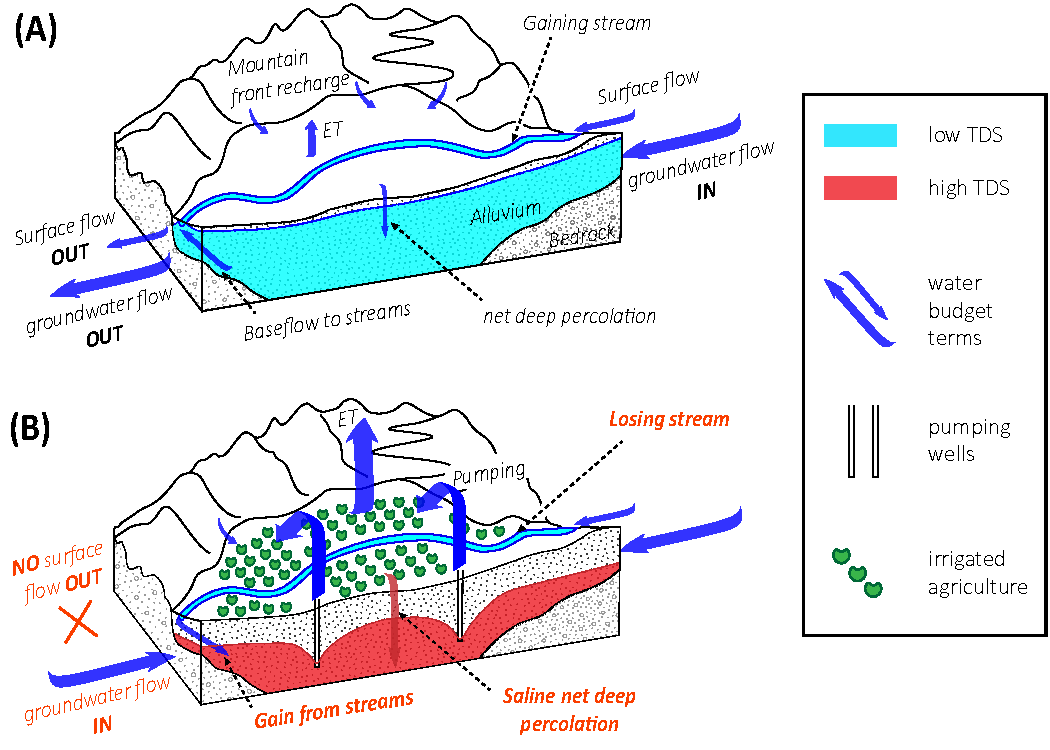
\includegraphics[width=\textwidth]{ch3_figs/mm_conceptual_model_gw_sal_2_stages.pdf}
	\caption{Conceptual model of ABCSAL. (A) Open basin, pre-groundwater development: surface and groundwater systems connect. Groundwater discharges dissolved solids into surface water which exits the basin. Groundwater at this stage is predominantly fresh (e.g., $<$ 1,000 mg/L). (B) Closed basin: groundwater pumping causes elimination of baseflow to streams. Lower groundwater levels cause subsurface inflow to drain adjacent basins. Pumped groundwater is concentrated by evapotranspiration (ET) when applied for irrigation. Salts migrate into the production zone of the aquifer, driven by vertical hydraulic gradients from recharge and pumping. Although these figures showtwo extremes (open and closed), partially-closed basins also exist.}
	\label{fig:conceptual_model_gw_sal}
\end{figure}


Importantly, we point out that the long-term continuous decline of groundwater storage is not a necessary condition for ABCSAL. Rather, even in basins where groundwater levels are stable and hence assumed to be free of overdraft, as long as they remain physically closed, they will salinate. Furthermore, although for simplicity we describe basins as either ``open" or ``closed", in reality, closure ranges from 0-100 \% (i.e., fully open to fully closed), and gradations of basin closure exist, which impact the rate of salinization and hence, the long-term temporal and vertical spatial salt distribution. Except for the most extremely exploited aquifers (one of which we explore in this study), many aquifers will fall somewhere between fully open to fully closed and not exactly at one extreme. 

In this research, we illustrate the development of ABCSAL in a historically open, freshwater basin using the agriculturally intensive Tulare Lake Basin (TLB) in California's southern Central Valley as a case study. Previous research in the TLB has shown evidence of salt accumulation in groundwater via simple water and salt budgets \citep{Kenneth1975}, and shallow aquifer salt accumulation from sediment dissolution processes in highly-soluble calcium and magnesium carbonates and sulfates \citep{Schoups2005}. Other studies have shown that TDS concentrations in TLB groundwater have increased over the last century \citep{Hansen2018, Lindsey2018}, and suggested this is the result of pumping for municipal and irrigation supply which has caused shallow, higher TDS groundwater to be driven downward into deeper aquifers. We are not aware of prior work that has placed these trends into the context of ABCSAL, or quantified potential rates of salinization across a range of aquifer depths and timescales. 

Our aim in this study is to assess the first order salt balance and timescales over which the TLB as a large production aquifer system becomes regionally degraded over most of the vertical extent of its nearly 200 $m$ thick main production zone. We conservatively assume that, under recent state regulation, groundwater overdraft is arrested, but not reversed. We compare timescales of ABCSAL degradation against the estimated lifespan of the greater Central Valley aquifer (i.e., 390 years at historical overdraft rates) \citep{Faunted.2009}, challenge the notion that the depletion of groundwater storage is a more urgent issue than the degradation of groundwater quality in the TLB (and in other basins with ABCSAL conditions), and consider the water management implications and the steps required to reverse extensive basin-scale groundwater salinization. The management would likely involve both hydrologic opening of the basin to provide natural outlets for salt, a reduction of sources of salinity, and the development of regional groundwater quality management models \citep{Fogg2006, CRWQCB2018}. The adaptation might involve the eventual desalination of most groundwater pumped from the basin, producing a future economic burden that should be anticipated and evaluated, as it bears on the security of water, food, and energy resources. 

This paper is organized as follows: first, we describe the hydrogeology, water budget, and water quality of the study site. Then we describe and justify our approach involving a simple 1D mixing cell solute transport model. Next, we present our results, and finally, we discuss the implications of the research, the limitations of our approach, and the extensibility of the study to other areas.  


%--------------------------------------------------------%
% Methods
%--------------------------------------------------------%
\section{Methods}

\subsection{Study area}
\label{ss_2_1}

In selecting the TLB as our study site, we looked for (1) a history of intensive groundwater pumping and irrigation, (2) availability of historical water budget and water quality data, and (3) social and economic significance. The TLB (Figure \ref{fig:tb_study_site}) occupies the southern third of the Central Valley, California and is bounded by the Coast Ranges to the west, the Tehachapi Mountains to the south, and the southern Sierra Nevada to the east. Geology strongly influences dissolved solid concentrations in the clastic sedimentary aquifer system composed of fluvial and alluvial fan deposits. Calcium and magnesium sulfates and carbonates in Coast Range sediment in the western TLB are more soluble than sediments from the predominately crystalline rocks of the Sierra Nevada to the east, thus the groundwater in the western basin tends to have higher TDS \citep{Fujii1995, belitz1990, deverel1988}. Fresh groundwater in the TLB spans depths from land surface to around 1,000 $m$ where brackish water and marine deposits limit the development of groundwater resources \citep{Program2010, Kang2016}. Above this deep brackish zone is a major freshwater aquifer system. In combination with a natural endowment of significant, but intermittent runoff from surrounding uplands, abundant fresh groundwater has transformed the TLB into one of the most heavily irrigated and economically productive agricultural regions in the world \citep{Hanak2011}. At its peak in the 1980s, approximately 14,164 $km^2$ of its 44,110 $km^2$ were irrigated \citep{TNC2014}. Today roughly 12,140 $km^2$ remain irrigated, with a total gross value of all agricultural crops and products at \$23.4 billion USD in 2017 \citep{kern2018, kings2018, fresno2018, tulare2018}. \\

% F:\Box Sync\Research\Post QE Research\DISSERTATION\01_mm\code\tb_study_site\tb_map.R
% tb_with_riv.pdf
% 01_mm\ai\study_site_water_budget.ai
% numbers come from archived (commented out Table 5)

\begin{figure}[H]
	\centering
	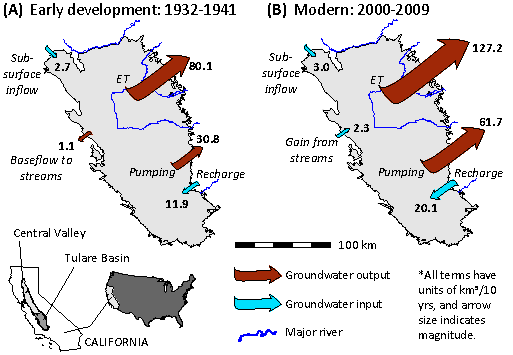
\includegraphics[width=.7\textwidth]{ch3_figs/study_site_water_budget_riv.pdf}
	\caption{The TLB overlies an agriculturally intensive sedimentary aquifer in California's southern Central Valley. Significant changes are observed in selected decadal hydrologic year water budget terms derived from C2VSim at (A) early-groundwater-development (not to be confused with pre-groundwater-development) and (B) post-groundwater-development timescales in the TLB. Notably, gaining streams transition to losing streams, and increases are observed in pumping, evapotranspiration (ET), and recharge (from diversions and natural sources, like streams, lakes, and watersheds). All terms are aggregated at the scale of the TLB, except for subsurface inflow, which is calculated at the northern TLB boundary. Note that this is not the TLB groundwater budget (Table \ref{tab_gwb}) nor the land surface and rootzone budget (SI Appendix Table \ref{ap_b_lsb}), but rather, a combination of ground and surface water budget terms that illustrate hydrologic change and show the main inputs (recharge) and outputs (pumping and evapotranspiration). Major rivers (shown in blue) from north to south include the San Joaquin, Kings, Kaweah, Tule, and Kern. Minor streams and tributaries are not shown.}
	\label{fig:tb_study_site}
\end{figure}

Although a TLB water budget from pre-development times is not available, the surface and subsurface hydrologic characteristics of the basin, which is a part of the larger Central Valley sedimentary basin (Figure \ref{fig:tb_study_site}), indicate that it was hydrologically open. We first discuss the surface hydrologic aspects. Despite the shallow topographic depression in which Tulare Lake used to exist, the freshwater lake periodically filled up and overflowed northward into the San Joaquin River \citep{grunsky1898irrigation, Davis1959}, providing an outlet for any accumulated salts. Reconstructions of historical Tulare Lake level indicate that in 19 of the 29 years from 1850 to 1878, it filled up and flowed out of the basin to the north \citep{USBR1970}. This water and salt exit via intermittent surface inundation would be different than, say, baseflow to a stream, but would accomplish the same flushing function. No overflows are documented after 1878 due to the diversion of tributary waters for agricultural irrigation and municipal water use \citep{ecorp2007}. 


\bgroup
\setlength{\tabcolsep}{1.3em}

% 01_mm_plots_tables.R in F:/ ... POst_QE_Research/DISSERTATION/01_mm
% average annual GW budget table - 1961-10-31 to 2001-09-30
% but a lot is added in the caption and table footnote, so beware changing this!!
% in MCMM.R:
% mg_to_metric_tons(sum(annual_fluxes$mass_flux[n]))/1e6, where n = the term desired

\centering
\begin{threeparttable}
	\begin{table}[H]
		\caption{Average annual groundwater and salt budget for the TLB (equation \ref{eq: gw_budget}) from C2VSim (1961-10-31 to 2001-09-30), and the modified no-overdraft budget used in this analysis (equation \ref{eq: gw_budget_mod}).}
	
		\begin{tabular}{rlrrrr}
			\label{tab_gwb}
			
			
			
			& \textbf{Source} & $\bm{Q \: \: (km^3/yr)}$ & $\bm{C \: \: (mg/L)}$ & $\bm{m \: \: (Metric \: Mtons)}$ & \\ 
			\hline
			\parbox[t]{2mm}{\multirow{8}{*}{\rotatebox[origin=c]{90}{\textbf{Historical budget}}}}
			& $R$ & 2.451 & 32.5 & 8.027E-02 & \\
			& $B$ & 0.236 & 32.5 & 7.475E-03 \\ 
			& $C$ & 0.572 & 32.5 & 1.852E-02 \\ 
			& $I$ & 0.011 & 32.5 & 3.250E-04 \\ 
			& $P$ & -6.761 & * & * \\ 
			& $N$ & 1.883 & * & * \\ 
			& $RWI$ & - & - & * & \\ 
			& $\Delta S$ & -1.608 &  &  \\ 
			
			\hline
			
			\parbox[t]{2mm}{\multirow{9}{*}{\rotatebox[origin=c]{90}{\textbf{Alternate budget}}}}
			& $R$ & 2.451 & 32.5 & 8.027E-02 & \\ 
			& $B$ & 0.236 & 32.5 & 7.475E-03 & \\ 
			& $C_{alt}$ & 0 & - & - & \\
			& $M$ & 0.678 & 32.5 & 2.204E-02 & \\ 
			& $I$ & 0.011 & 32.5 & 3.250E-04 & \\ 
			& $P_{alt}$ & -5.259 & * & * & \\ 
			& $N$ & 1.883 & * & * & \\ 
			& $RWI$ & - & - & * & \\ 
			& $\Delta S_{alt}$ & 0 & - & - & \\ 
			\hline
			\multicolumn{4}{l}{\scriptsize{* non-constant term calculated at each time step}} 
		\end{tabular}
		
		
		$Q$ is the volumetric flow rate, $C$ is the concentration of TDS, and $m$ is the mass of salt. Groundwater budget terms are:
		%$W$ = stream gain, 
		$R$ = recharge from streams, lakes, and watersheds, 
		%$L$ = lake gain,
		$B$ = lateral mountain front recharge from streams and watersheds,
		$C$ = subsidence flow,
		$C_{alt}$ = subsidence flow to eliminate overdraft (along with $M_{alt}$ and $P_{alt}$),
		$M$ = managed aquifer recharge to eliminate overdraft (along with $C_{alt}$ and $P_{alt}$), 
		$I$ = subsurface inflow from the north,
		$P$ = groundwater pumping,
		$P_{alt}$ = alternate groundwater pumping to eliminate overdraft (along with $M$ and $C_{alt}$),
		$N$ = net deep percolation (recharge from the land surface through vadose zone and into saturated groundwater),
		$RWI$ are rock-water interactions.
		$\Delta S$ = change in groundwater storage.
		$\Delta S_{alt}$ = change in groundwater storage for the modified budget. 
		The modified budget eliminates overdraft by reducing $P$ to $P_{alt}$ according to equation (\ref{eq: pumping_in_cells}), and introducing recharge $M$. 
		
	\end{table}
	
\end{threeparttable}

\egroup

\clearpage


The subsurface characteristics also indicate open hydrologic conditions. There is significant evidence that groundwater flowed northward into the adajacent San Joaquin Basin in pre-development times (circa early 1900s). This evidence includes (1) historical measurements of Central Valley groundwater TDS showing lowest TDS values in the TLB, with increasing TDS to the north into the San Joaquin Basin \citep[Table 23]{mendenhall1916ground}, consistent with northward groundwater flow and the accompanying down-hydraulic-gradient groundwater chemistry evolution that is routinely observed in sedimentary basins, e.g., \citep{palmer1984geochemical}; (2) the regional, south-to-north topographic gradient to provide the driving force for gravity-driven flow in the same direction, out of the TLB, even if there existed shallower, local groundwater flow components from north to south at the subtle depression that collected Tulare Lake (e.g., refer to classic work of \cite{toth1970conceptual} on topographically controlled, gravity-driven flow systems); and (3) horizontal stratification of fine- and coarse-textured sediments in the Central Valley sedimentary basin that results in much lower effective hydraulic conductivities in the vertical direction than the horizontal e.g., \citep{weissmann2002dispersion, Faunted.2009}, thereby minimizing influence of subtle topographic features like the Tulare Lake depression on all but the shallowest groundwater flow components (e.g., refer to \cite{toth1970conceptual} and related work).

Summarizing, our conceptual model of the pre-development TLB hydrologic system is one in which the subtle topographic depression that collected the typically 12 $m$ deep Tulare Lake \citep{preston1990tulare}, together with the periodic overflow of the lake and discharge to the north, resulted in a partly open surface drainage system. Further, the larger topographic and geologic structure of the basin, together with groundwater chemistry evidence, indicates there was net-northward groundwater flow, making the TLB groundwater system an open hydrologic basin in pre-development times.

Parts of TLB may have been salinating to some degree before development due to shallow evaporation of groundwater and surface water (case (3) in Introduction), in contrast to the ABCSAL process that we describe in this paper. Portions of the TLB closed under pre-development conditions would lead to salt accumulation in and near its playas (e.g., Buena Vista Lake, Tulare Lake): an evaporative boundary of the basin and endpoint to all surface water discharge (case (2) above). This is consistent with observations of high salinity near and in these lakebeds \citep{Hansen2018, Fujii1995}. Although there exist local areas of shallow groundwater with elevated salinity on the west side of the TLB, these areas are typically associated with salt mobilization out of alluvial sediments originating from marine sedimentary source rocks in the Coast Ranges, and not from basin closure.

By the time regional groundwater levels were mapped in the early twentieth century, the TLB showed signs of closure: groundwater flow across the northern boundary was minimal, and flowed north to south, into the TLB \citep{mendenhall1916ground, ingerson1941hydrology}. Although pre-groundwater-development (pre-1850) water budgets are unavailable, two large-scale, regional groundwater flow models of the Central Valley \citep{Brush2013, Faunted.2009} provide decadal groundwater budgets for early- (1932-1941) and post-groundwater-development (2000-2009) timescales.

Relative to the decadal hydrologic water year budgets of early-groundwater-development, post-groundwater-development water budgets show much higher pumping, crop evapotranspiration, and recharge \citep{Brush2013}. As groundwater levels fell, gaining streams transitioned to losing streams, and subsurface inflow along the northern basin boundary slightly increased (Figure \ref{fig:tb_study_site}). Groundwater discharge to surface water almost entirely ceased. Surface water exits the basin in rare years when the Kings, Kaweah, and Kern rivers produce sufficiently large floods, mostly runoff from the surrounding uplands. Evapotranspiration from irrigated crops has become the dominant water outflow, and this flow is much greater than it was during early-groundwater-development \citep{Brush2013}. Taken together, these hydrologic changes have transitioned the TLB into an anthropogenically closed groundwater system with commensurate onset of ABCSAL.  




%
%---------------- MODEL DEVELOPMENT ------------------%
%
\subsection{Mixing Cell Model Development}
\label{ss_2_3}

Given the large space and time scales of interest, and the large-scale effectively one-dimensional vertical flow conditions in the basin due to pumping and recharge, we used a lumped parameter approach based on upscaling water fluxes of a fully three-dimensional groundwater model. % was employed as an appropriately parsimonious modeling tool. 
Although local hydrogeologic conditions vary and can lead to locally complex three-dimensional flow and transport, our focus here is on large scale salinization behavior and time scales, thus an upscaled model was appropriately parsimonious. %which is well-captured with a one-dimensional approach. %We assess results against existing fully three-dimensional flow and salt transport models that also address aquifer heterogeneity, albeit at spatial scales significantly smaller than the TLB, to ascertain the appropriateness of the mixing cell approach chosen here.
Moreover, upscaling the advection dispersion equation to regional scales remains a scientific and computing challenge \citep{guo2019adaptive, guo2019upscaling} beyond the scope of this study.

Mixing cell models, also called discrete-state compartment models, are computationally inexpensive and have successfully been used in place of complex flow models to provide rapid, first-order estimates of water budgets, mass flux, and contaminant concentrations \citep{Campana1975, Campana1984, Campana1987, Carroll2008, Kirk1990}. A mixing cell approach segments the system into a set of control volumes. In each time step of the model, water and salt masses are passed between the cells, and new concentrations are calculated at each cell. Here, we represent the TLB groundwater system through a one-dimensional, vertical column of discrete control volumes (cells), given the predominance of vertical downward flow at the aquifer system scale. We assume that each cell consists of a fraction $f$ of sediments participating in groundwater flow and salt transport with porosity $\eta$. We neglect flows and rock-water interactions in sediments not participating in transport, of proportion $1-f$ (more details below). The thickness of each cell is chosen such that the advective travel time ($\Delta t$) of water and salt downward through each cell is exactly 50 years (synchronized tipping bucket model, see equation \ref{eq: discretization}) below, thus full mixing occurs at each cell even as the groundwater flow velocity decreases with depth. To determine the mixing cell parameters, water fluxes throughout the vertical domain (e.g., recharge, vertical flow rate, pumping) are obtained by averaging (i.e., mass-conservative upscaling) the TLB portion of a fully three-dimensional, heterogeneous groundwater flow model of the Central Valley \citep{Brush2013}.  

The salt accumulation in a mixing cell at a discrete time $k$ is a mass balance of the initial mass ($m_k$) $[M]$, incoming mass ($m_k^{in}$) and exiting mass ($m_k^{out}$).  

\begin{equation}
m_{k+1} = m_k + m_k^{in} - m_k^{out}
\label{eq: mass_balance}
\end{equation}  

Input and output mass terms can be calculated for each term in the water and salt budget (Table \ref{tab_gwb}), from their input and output concentration ($C_k^{in}$, $C_k^{out}$ $[ML^{-3}]$) and input and output volumetric flow ($Q_k^{in}$, $Q_k^{out}$ $[L^3]$):

\begin{equation}
m_k^{in} = C_k^{in} Q_k^{in}   \: \: ; \: \:  m_k^{out} = C_k^{out} Q_k^{out}
\label{eq: m_in_cell}
\end{equation}

Finally, the concentration in a mixing cell at time step $k$ is:

\begin{equation}
C_{k+1} = \frac{m_k + m_k^{in} - m_k^{out} + \rho V}{V f \eta}
\label{eq: c_in_cell}
\end{equation}


where $V$ $[L^3]$ is the total cell volume, $f$ $[-]$ is the fraction of sediments actively participating in groundwater flow and salt transport, $\eta$ $[-]$ is the porosity of those sediments, and $\rho$ $[ML^{-3}]$ is rock-water interaction coefficient. The fraction $f$ is found to be 0.99 \citep{Brush2013}, which in the C2VSim model includes all textures but the Corcoran clay, a relatively impermeable clay layer comprising around 1\% of the model volume. Porosity, $\eta$, is set to 0.40, the average for the TLB. Coarse and fine sediment porosities do not appreciably differ, averaging around 0.40 with an interquartile range of 0.39 - 0.41 for all textures, as demonstrated in abundant core analyses \citep{Johnson1968}, and discussed further in SI Appendix Table \ref{ap_b_porosity_boot} and Figure \ref{ap_b_porosity_boot_hist}; hence, we did not consider varying $\eta$ across aquifer layers. 

To account for mass contribution from natural dissolution of geologic minerals, we define a zero order source term called the rock-water interaction coefficient $\rho$ $[ML^{-3}]$. Rock dissolution along groundwater flow paths is well documented in sedimentary aquifers \citep{palmer1984geochemical, oetting1996regional, toth1999groundwater, mahlknecht2004groundwater, cloutier2008multivariate}. We obtain a representative mass dissolution rate from the slope of a representative TDS profile for the TLB from land surface to the base of fresh water \citep{Williamson1989, Kang2016}. The product of the rock-water interaction coefficient $\rho$ and the cell volume ($V$) is the additional mass accumulated from rock-water interactions in the cell. We also evaluate an alternative scenario with $\rho =$ 0. 

We solve (\ref{eq: c_in_cell}) sequentially over the stacked mixing cells from top to bottom and across seven 50-year time steps from 1960 (initial condition) to 2310 (synchronized tipping bucket approach) to obtain the variation of salinity with depth and time. 

The discretization, $\Delta z_j$, of the stacked series of mixing cells (Figure \ref{fig:conceptual_model_mm}) is driven by the time step, $\Delta t$ = 50 years, and the representative basin-scale vertical Darcy velocity, $q_j$, within the $j^{th}$ mixing cell:

\begin{equation}
\Delta z_j =  \frac{q_j}{f \eta}  \cdot  \Delta t
\label{eq: discretization}
\end{equation}

Since $q_j$ is depth dependent, we solve (\ref{eq: discretization}) sequentially for $j$ = 1...m, beginning at the water table to compute the vertical discretization of the stacked mixing cell model. Here, we assume that the inflow into a mixing cell, $q_{j-1, j}$ is representative of the flow rate $q_j$ throughout the cell. Thus -- to compute cell thicknesses with equation (\ref{eq: discretization}) -- the pumping, $P_j$, lateral basin flow $I_j$, or subsidence flow $C_j$ (Figure \ref{fig:conceptual_model_mm}) conceptually flow into or out of the mixing cell bottom. The following sections provide further details on the parametrization of (\ref{eq: c_in_cell}) and (\ref{eq: discretization}).

\begin{figure}[H]
	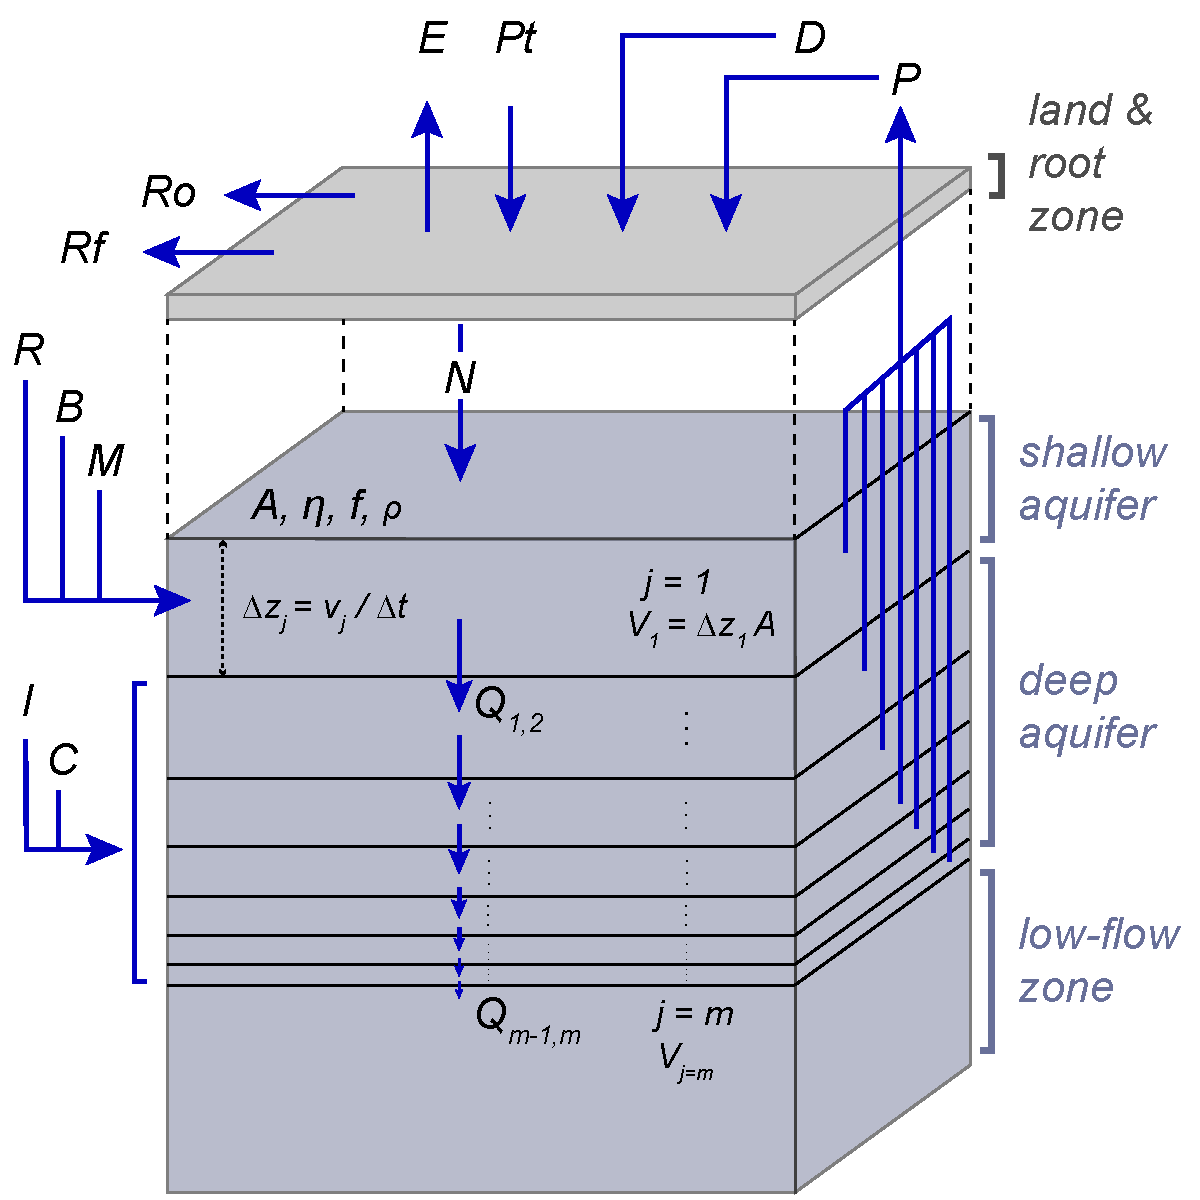
\includegraphics[width=\textwidth]{ch3_figs/mm_conceptual_model.pdf}
	\caption{Conceptual land-rootzone model and groundwater mixing cell model with surface area $A$, porosity $\eta$, aquifer fraction $f$, rock-water interaction coefficient $\rho$, and $m$ cells. The cell thickness $\Delta z_j$ is given per equation (\ref{eq: discretization}), where average linear velocity $v_j$ = $q_j / f \eta$. The cell volume $V_j$ is the total bulk volume of the rock including aquifer and non-aquifer material. The TDS in cell $j$ is calculated by equation (\ref{eq: c_in_cell}). The land and root budget (SI Appendix Table \ref{ap_b_lsb}) accounts for pumping ($P$), surface water diversions ($D$), precipitation ($Pt$), evapotranspiration ($E$), runoff ($Ro$), return flow ($Rf$), and net deep percolation ($N$). $N$ enters the top of the groundwater mixing cell model along with recharge from streams, lakes, and watersheds ($R$), boundary inflow from mountain front recharge ($B$), and managed aquifer recharge ($M$). Internal flows from subsurface inflow from the north ($I$), subsidence flow ($C$), and pumping ($P$) are distributed proportional to cell volume, e.g., equation (\ref{eq: pumping_in_cells}). The average annual groundwater and salt budget is reported in Table \ref{tab_gwb}.}
	\label{fig:conceptual_model_mm}
\end{figure}



%
%---------------- BOUNDARY CONDITIONS ------------------%
%
\subsection{Boundary conditions, model parameters, and stochastic simulation}
\label{ss_2_4}

Initial conditions, boundary conditions, and model parameters are informed by the C2VSim groundwater flow model developed by the California Department of Water Resources \citep{Brush2013}, publicly available water quality data \citep{CSWRCB}, and previous field studies of the TLB. The following describes methods used to determine (1) water and salt budgets, (2) salt fluxes from evaporative concentration and pumped groundwater, (3) the groundwater velocity-depth profile, (4) the initial TDS-depth profile, and (5) spatial parameters and aquifer properties. Lastly, we discuss the simulation timescale and the role of stochastic simulation.

%
%---------------- SALT/WATER BUDGETS ------------------%
%
\subsubsection{Water and salt budgets}
\label{ss_2_5}

The water budget is based on C2VSim version 3.02, a 3 layer and 1,392 element, regional scale, finite-element groundwater flow model of California's Central Valley alluvial aquifer system \citep{Brush2013}. C2VSim is an application of the Integrated Water Flow Model (IWFM) \citep{Dogrul2018}, a water resources management and planning model that simulates surface water, stream-groundwater interaction, vadose zone flow, and groundwater flow. In the C2VSim model, California's Central Valley aquifer is separated into 21 subregions, and detailed land surface, root zone, and groundwater budgets for each subregion are calculated at monthly time steps from the 1923 to 2009 hydrologic years. The TLB is represented by subregions 14-21. Because of its detailed representation of surface-groundwater interaction, groundwater pumping, three-dimensional aquifer structure, and calibration, C2VSim was chosen as a reasonable representation of the TLB water budgets, groundwater velocities, and thus chosen to develop the mixing cell model. 

The C2VSim model was run for the 40-year period from 1961-10-31 to 2001-09-30 to obtain an average annual TLB groundwater budget (an equivalent average annual landscape/root zone budget is provided in SI Appendix Table \ref{ap_b_lsb}). This post-groundwater development water management time frame is characterized by pumping and overdraft, in addition to wet, dry, above normal, below normal, and critical water year types. The C2VSim change in groundwater storage is defined as:

\begin{equation}
\Delta S = R + B + C + I + N - P
\label{eq: gw_budget}
\end{equation}

where $\Delta S$ is change in groundwater storage [$L^3$], $R$ is basin recharge from streams, lakes, and watersheds [$L^3$], $B$ is lateral mountain front recharge from streams and watersheds [$L^3$], $C$ is subsidence based flow from clay compaction [$L^3$], $I$ is subsurface inflow from the north [$L^3$], $N$ is net deep percolation predominately from irrigation water [$L^3$], and $P$ is groundwater pumping [$L^3$]. The dominant budget terms are $P$, $R$, and $N$ (Table \ref{tab_gwb}). 

To demonstrate ABCSAL under long-term conditions that avoid further overdraft (but not basin closure), we solve the mixing cell model equations (\ref{eq: c_in_cell}) - (\ref{eq: discretization}) alternatively for $\Delta S_{alt}$ = $\Delta C_{alt}$ = 0. Overdraft is eliminated with an alternate budget (Table \ref{tab_gwb}), which adds managed aquifer recharge, $M$ as inflow to the top mixing cell (Figure \ref{fig:conceptual_model_mm}), and reduces pumping to an alternative pumping level, $P_{alt}$. We add $M$ = 0.68 $km^3$, which was determined by a prior study as the maximum theoretical recharge available to the San Joaquin Valley (which includes the TLB), assuming unlimited infrastructure and water transfer ability \citep{Hanak2019}. Eliminating overdraft in this way effectively maintains a steady-state, saturated model that remains closed to due to lack of baseflow and groundwater outflow. Hence, the water level is immobile, but the salt front can move, thus simulating salt migration without drying out cells due to overdraft.

Since $M$ represents captured surface water flow, we assign it the same TDS as natural water (32.5 $mg/L$), discussed below. We also simulated $M$ with a TDS of 0 $mg/L$ (SI Appendix Table \ref{ap_b_p_sim_m_with_tds_0}
) and found that it had a negligible impact on resulting salt concentrations presented in this study (SI Appendix Table \ref{ap_b_p_sim}). 

The alternate, reduced pumping $P_{alt}$, is computed by rearranging (\ref{eq: gw_budget}), adding $M$, and setting $\Delta S_{alt}$ = $C_{alt}$ = 0:

\begin{equation}
P_{alt} = R + B + M + I + N 
\label{eq: p_alt}
\end{equation}

%[THE FOLLOWING ONLY IF YOU WERE TO USE YOUR CURRENT RESULTS FROM 2010 AS INITIAL CONDITIONS FOR YOUR RUNS USING (6) FOR THE PERIOD FROM 2010 to 2265:]
%We use (5) to simulate the historic period 1960-2010, and the resulting concentration profile as initial condition for using (6) to solve for flow and transport conditions from 2010 - 2265.

Therefore, the modified no-overdraft alternate groundwater budget is:  

\begin{equation}
\Delta S_{alt} = R + B + C_{alt} + M + I + N - P_{alt} = 0
\label{eq: gw_budget_mod}
\end{equation}


The salt budget is calculated by assigning a TDS concentration to each term in the groundwater budget (\ref{eq: gw_budget_mod}). TDS for natural waters (e.g., stream, lake, and managed aquifer recharge budget terms) were determined to be 32.5 $mg/L$, by computing the median of the sampling distribution of sample TDS medians in TLB stream samples \citep{nwis} from 1951 - 2019 (SI Appendix Figure \ref{ap_b_nat_waters} and Table \ref{ap_b_gw_and_sw_c_summary}). Similarly, the TDS of diverted surface water was calculated to be 264.5 $mg/L$, as the average annual water and salt budget from 1985 - 1994 of two major surface water conveyance structures, the California State Water Project and the State Water Project \citep{Cismowski2006} (SI Appendix Table \ref{ap_b_gw_and_sw_c_summary}). Salt and water budgets are detailed in Table \ref{tab_gwb}. 


%
%---------------- VELOCITY DEPTH PROFILE ------------------%
%
\subsubsection{Velocity-depth profile}
\label{ss_2_6}

To explicitly solve for the mixing cell discretization (\ref{eq: discretization}), we fit a linear model to the C2VSim vertical Darcy velocities, reported for each finite element cell in the three layer C2VSim grid at the layer-to-layer boundaries. Due to increases in recharge and pumping caused by groundwater development and irrigation, the groundwater flow system is vertically dominant, and thus supports the application of a 1D, vertically oriented model. To account for groundwater velocity change in the alternate groundwater budget (\ref{eq: gw_budget_mod}), groundwater velocity is scaled proportional to the decrease in vertical volumetric flow rate, $P_{alt}/(P + C)$ = 0.85 (a 15 \% reduction). This is equivalent to the ratio of net downward volumetric flow in the alternate budget to the net downward volumetric flow in the historical budget (Table \ref{tab_gwb}). 

\begin{equation}
q(z) = (\beta_0 + \beta_1 z) \cdot \frac{P_{alt}}{P+C}
\label{eq: vel}
\end{equation}

where $\beta_0$ and $\beta_1$ are the regression coefficients (SI Appendix Table \ref{ap_b_velocity_coefficients}), and the overall change (reduction) in velocity is -15\%. Mixing cell thickness (\ref{eq: discretization}) is determined by computing $q_j$ from (\ref{eq: vel}) for the depth, $z$, of the bottom of the mixing cell $j-1$ (top of cell $j$). To ensure consistency between the water balance terms in (\ref{eq: gw_budget}) and the approximated vertical velocity profile (\ref{eq: vel}), we compute the water mass balance error, $MB_{error, j}$, for each mixing cell $j$:

\begin{equation}
MB_{error, j} = q_{j-1,j} + I_j - P_{alt,j} - q_{j,j+1}
\label{eq: mb_error_inside}
\end{equation}

For the uppermost mixing cell $j$ = 1, we rearrange (\ref{eq: mb_error_inside}), replacing $q_{j-1,j}$ for the sum of $N$, $R$ and $B$, and ignoring subsurface inflow $I_j$ (Figure \ref{fig:conceptual_model_mm}):

\begin{equation}
MB_{error, 1} = N + R + B + M - P_{alt,1} - q_{1,2}
\label{eq: mb_error_top}
\end{equation}

The cell by cell budget and mass balance errors (which are effectively zero, and equivalent to the cell-by-cell change in storage) are reported in SI Appendix Table \ref{ap_b_cbc}.


%
%---------------- EVAPOCONCENTRATION ------------------%
%
\subsubsection{Evapoconcentration and pumping}
\label{ss_2_7}

Evapotranspiration removes a majority of total applied water, leaving behind dissolved solids in the crop rootzone that eventually migrate into groundwater. We model the evapoconcentration of TDS in total applied water (a combination of pumped groundwater and imported surface water diversions) by accounting for the application efficiency \citep{burt1997irrigation}, and thus the fraction of water that remains after evapotranspiration:  

\begin{equation}
C_N = \left( \frac{m_D + m_P}{V_D + V_P} \cdot \frac{1}{1 - E_a} \right) = \frac{C_{D,P}}{1 - E_a}
\end{equation}

$C_N$ is the concentration of net deep percolation after accounting for evapotranspiration. $m_D$ and $m_P$ are the mass, and $V_D$ and $V_P$ are the volume of surface water diversions ($D$) and pumping ($P$), respectively. $C_{D,P}$ is the concentration of total applied water from surface water diversions and pumping (calculated by mixing diversions and pumped groundwater in their respective proportions, see SI Appendix Table \ref{ap_b_velocity_coefficients}), and $E_a$ is the application efficiency, which has a measured regional average of 0.78 in the Tulare Basin \citep{sandoval2013spatial}, and agrees with measured values in hydrologically similar areas \citep{hanson1995, howell2003irrigation}. Alternatively, the C2VSim landscape/soil water budget (SI Appendix Table \ref{ap_b_lsb}) provides an application efficiency, $E_a$, of 0.88 when considering the amount of water infiltrating into the soil and deep percolation. For sensitivity analysis, we run simulations for several $E_a$ between 0.78 and 0.88 to further explore model outcome uncertainty.

For the stacked mixing cell model, we assume that $P_{alt}$ in the no-overdraft groundwater budget (\ref{eq: p_alt}) is distributed uniformly with depth, from the water table to the last mixing cell $m$. Similarly, we assume lateral inflow $I$ is uniformly distributed across depth, from cell 2 to cell $m$. Therefore, pumping is proportional to mixing cell thickness, and the salt mass flux due to pumping during time step $k$ in mixing cell $j$ is:

\begin{equation}
m_{j,k} = \frac{V_j f \eta}{f \eta \sum_{i=1}^{n} V_i} P C_{j,k}
\label{eq: pumping_in_cells}
\end{equation}

Noting that the $f \eta$ term drops out, and summing over all mixing cells at time $k$ gives the total mass flux from groundwater pumping ($m_{P, k}$):  

\begin{equation}
m_{P, k} = \sum_{j=1}^{n} \frac{V_j}{\sum_{i=1}^{n} V_i} P C_{j, k}
\end{equation}




%
%---------------- INITIAL CONCENTRATION ------------------%
%
\subsubsection{Initial TDS-depth profile}
\label{ss_2_8}

The initial TDS-depth profile is determined by fitting a linear model to the pre-1960 TDS-depth measurements (Figure \ref{fig:predev_tds_bc}) \citep{CSWRCB}. Due to the influence of freshwater recharge at the land surface and rock-water interactions, pre-1960 TDS generally increases with depth, consistent with observations of increasing TDS with depth in the region \citep{Kang2016, Kharaka1992, Program2010}. \\  

% in F:\Box Sync\Research\Post QE Research\DISSERTATION\01_mm\code\02_reanalyze_gw_tds.R
% search predev_tds_bc.pdf
% edited in ai/predev_tds_bc.ai
\begin{figure}[H]
	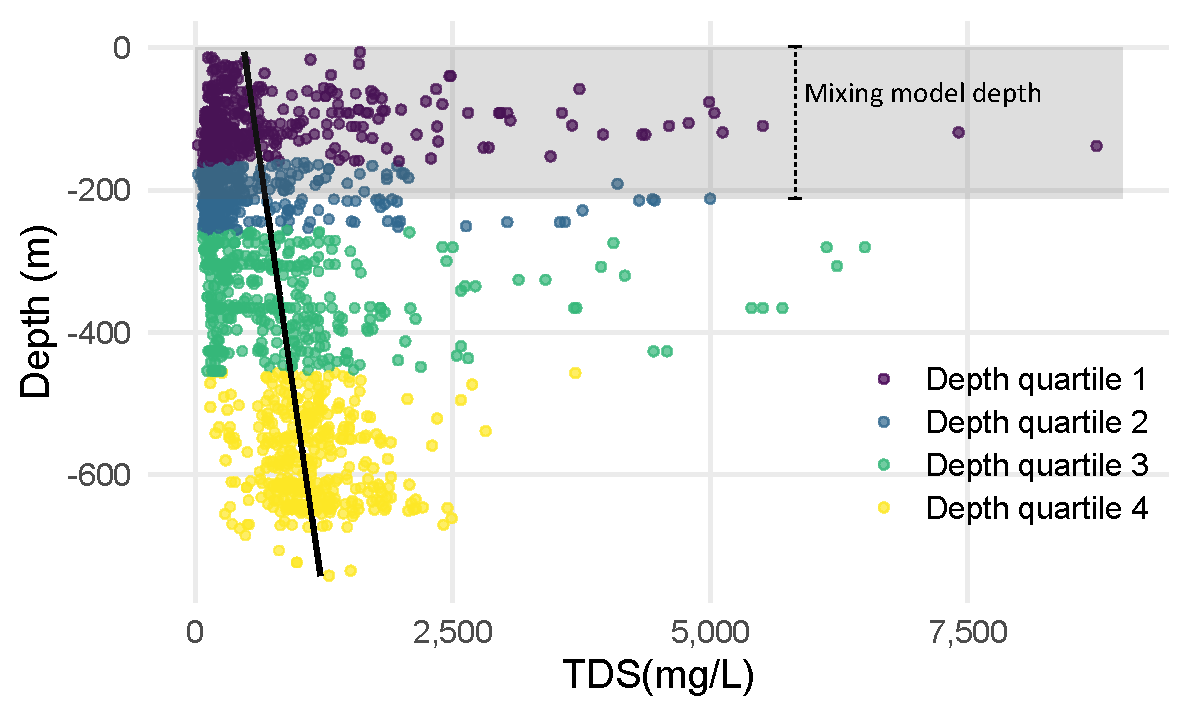
\includegraphics[width=\textwidth]{ch3_figs/predev_tds_bc.pdf}
	\caption{Pre-1960 groundwater quality generally decreases with depth, reaching an average concentration of 1,000 mg/L at 526 $m$ deep. The initial TDS-depth concentration at $t$ = 0 is approximated by a linear model, shown as a black line. The transparent, grey rectangle shows the depth of the mixing cell model (212 $m$).}
	\label{fig:predev_tds_bc}
\end{figure}


%
%-------- ENSEMBLE SIMULATION ------------%
%
\subsubsection{Ensemble simulation}
\label{ss_2_9}

We assign a uniform probability distribution to the parameters of which we are least certain and discrete values to those that are measured (SI Appendix Table \ref{ap_b_geometry}), then perform Monte Carlo simulation to generate an ensemble output. The mixing cell model is evaluated 1,000 times -- which the computational simplicity of a lumped model permits; modeling uncertainty in this way with a distributed parameter, 3D flow and transport model would be computationally prohibitive. Parameter ranges are estimated from literature for rock-water interaction coefficient \citep{Williamson1989, Kang2016}, detailed in section \ref{ss_2_3}. As described in section \ref{ss_2_7}, application efficiency is both measured \citep{sandoval2013spatial}, and calculated from C2VSim \citep{Brush2013}.  

To show the influence of rock-water interactions on the progression of closed basin salinization, we simulate two basic scenarios:  

\begin{enumerate}
	\item No rock-water interactions: mass accumulates from water budget inputs.  
	\item Rock-water interactions are present: mass accumulates from water budget inputs, but also internally via rock-water interactions (see section \ref{ss_2_3} for details).  
\end{enumerate} 




%--------------------------------------------------------%
% Results
%--------------------------------------------------------%

\section{Results}
\label{s_3}

%
%----------- GW and SALT BUDGET ---------------%
%
\subsection{Groundwater and salt budget}
\label{ss_3_1}

The average historical C2VSim groundwater budget in the TLB from 1961-10-31 to 2001-09-30 (Table \ref{tab_gwb}) reflects post-groundwater development conditions. Pumping removes an average of -6.76 $km^3/yr$ from the groundwater system. Natural recharge from streams, lakes, and watersheds adds an average of 2.45 $km^3/yr$, and net deep percolation of agricultural irrigation adds an average of 1.89 $km^3/yr$. Smaller sources of water inflow include subsidence flow (0.57 $km^3/yr$), lateral mountain front recharge from streams and watersheds (0.24 $km^3/yr$), and subsurface inflow from the north (0.01 $km^3/yr$). 

The alternate budget (Table \ref{tab_gwb}) used in this study eliminates overdraft ($\Delta S$ = 0), and is identical to historical budget described above, except that pumping $P_{alt}$ is reduced to -5.26 $km^3/yr$, managed aquifer recharge $M$ is added at a rate of 0.68 $km^3/yr$, and subsidence flow $C_{alt}$ is reduced to 0. Importantly, in this alternative budget the basin remains closed.

Salt inputs to the system (Figure \ref{fig:salt_ec}A) come from pumped groundwater, water budget terms, and rock-water interactions.


Groundwater pumping for agriculture is unlike other water budget terms ($I, M, R, B$) and rock-water interactions in that it does not \textit{add} new salt into the system, but rather \textit{recycles} existing salt from deeper layers to the land surface and back into shallow groundwater via irrigation (discussed in Section \ref{ss_3_3}). In the no rock-water interactions scenario ($\rho = $ 0), the median mass recycled by pumped groundwater exceeds the mass input of all other water budget terms by a factor of 1.7 to 3.5
% MCMM.R df5$m[c(43,49)]/(df5$m[c(36,41)] + df5$m[c(29,35)])
depending on the timeframe considered. When rock-water interactions are present ($\rho > $ 0), they initially contribute a comparable mass to groundwater pumping (around 4 metric $Mtons$), but with time, salt accumulates in the aquifer, and the mass recycled by groundwater pumping exceeds the mass imparted by rock-water interactions (Figure \ref{fig:salt_ec}A). 

Annually, surface water diversions add 1.5 
% MCMM.R   df5$m[1]/1e6
metric $Mtons$ of salt to the study site. This is around 4
% MCMM.R   (df5$m[1]/1e6 ) / (df5$m[8]/1e6)
times the amount of all other non-pumping water budget terms combined ($I, M, R, B$), which add only 0.35 
% MCMM.R   df5$m[8]/1e6
metric $Mtons$. We estimate that rock-water interactions add between 3.3 metric $Mtons$ and 4.6
% MCMM.R   c(df5$p5[22], df5$p95[28])/1e6
metric $Mtons$ of salt annually. This exceeds the mass introduced by imported surface water and is comparable to the mass recycled by groundwater pumping. 


% in Github/Monte-Carlo-Mixing-Model/code/MCMM.R
% search p23.pdf
\begin{figure}[H]
	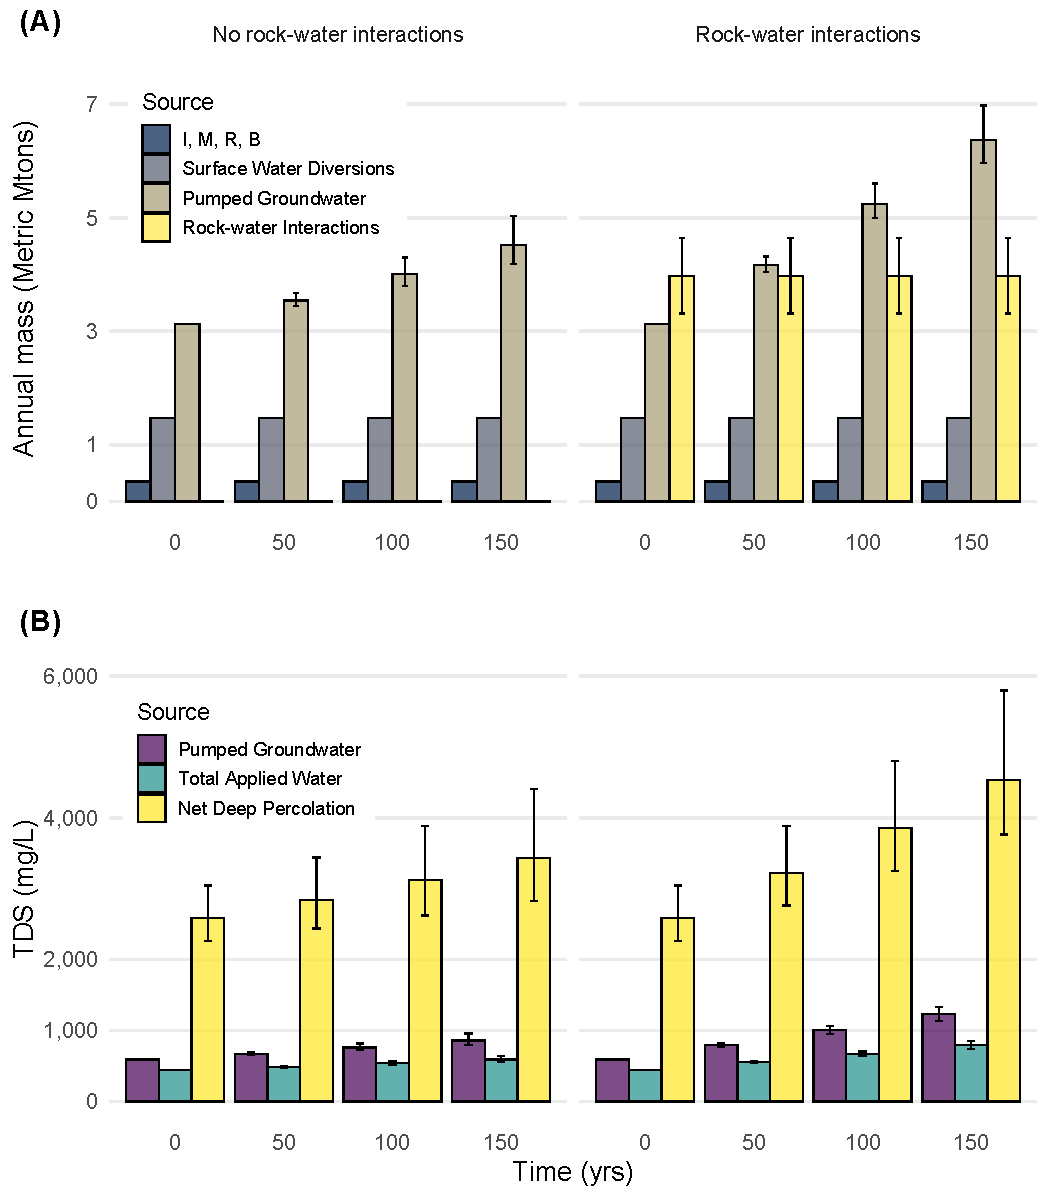
\includegraphics[width=\textwidth]{ch3_figs/p23.pdf}
	\caption{Annual mass flux and TDS of selected budget terms. The height of each column is the ensemble median result, and the width of error bars, if present, is the interquartile range of the ensemble distribution. (A) Pumped groundwater contributes more mass than surface water diversions and all other water budget terms combined (represented by their symbol: $I, W, R, B$). (B) TDS of \textit{pumped groundwater} is diluted when mixed with imported surface water, which forms \textit{total applied water}. However, evapotranspiration concentrates total applied water, which enters the groundwater system as \textit{net deep percolation}. Over time in a closed basin system, the groundwater salinates, which in turn increases the concentration of total applied water and net deep percolation. }
	\label{fig:salt_ec}
\end{figure}



Due to the closed-basin hydrology of the study site, there are no exits for salt to leave the system. Instead, pumping and irrigation recycle salts within the basin, and evapotranspiration by crops at the land surface increases the concentration of net deep percolation, which recharges groundwater (Figure \ref{fig:salt_ec}B). 

Evapoconcentration by crops at the land surface increases the average concentration of total applied water (pumped groundwater combined with surface water diversions) by 5.1 - 6.8
% (filter(EC_dat2, time == 0 & legend == "C") %>% slice(1) %>% .$p5 ) / (filter(EC_dat2,time == 0 & legend == "B") %>% slice(1) %>% .$p95 ) 
% (filter(EC_dat2, time == 0 & legend == "C") %>% slice(1) %>% .$p95 ) / (filter(EC_dat2,time == 0 & legend == "B") %>% slice(1) %>% .$p5 ) 
times its original amount, regardless of whether rock-water interactions are absent or present. As previously discussed, since pumped groundwater concentration increases with time, total applied water and thus net deep percolation also become increasingly saline over time.  




%
%----------- GW SAL EVOLUTION ---------------%
%
\subsection{Progression of groundwater salinization}
\label{ss_3_3}

The shallow aquifer (36 $m$) is heavily impacted by the recycling of salts via pumping and irrigation, and exceeds the freshwater concentration threshold (1,000 $mg/L$) within decadal timescales (Figure \ref{fig:p_sim}). Intermediate (132 $m$) and deep aquifers (187 $m$) exceed 1,000 $mg/L$ within century-long timescales. \\

% in Github/Monte-Carlo-Mixing-Model/MM_no_RWI.Rmd
% search p_sim.pdf
% edited in AI in DISSERTATION/01_mm/ai/p_sim_both2.ai
\begin{figure}[H]
	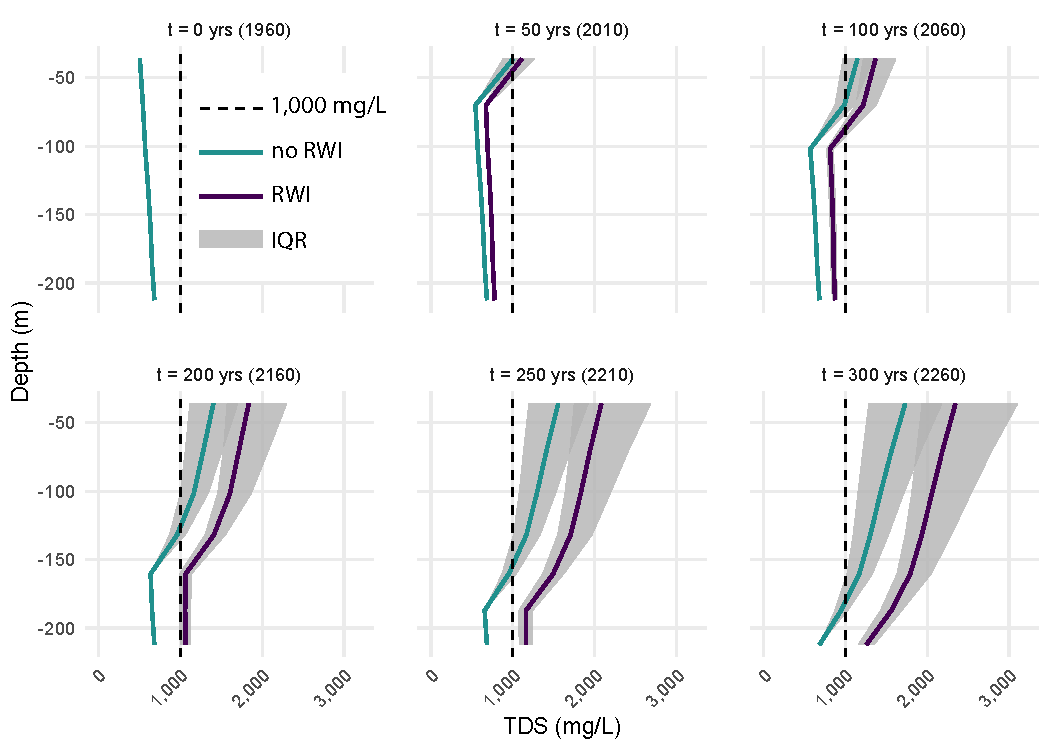
\includegraphics[width=\textwidth]{ch3_figs/p_sim_both2.pdf}
	\caption{Progression of groundwater salinization ensemble results for two scenarios (with and without rock-water interactions). RWI stands for rock-water interactions. The blue and purple lines show the ensemble median concentration for the two scenarios, and the interquartile range (IQR) of the ensemble simulations is shown as a grey shaded area. Complete statistics are provided in SI Appendix Table \ref{ap_b_p_sim}.}
	\label{fig:p_sim}
\end{figure}


Uncertainty in the salt balance results from parameter uncertainty expressed in the Monte Carlo simulation (section \ref{ss_2_9}), which affects the distribution of calculated salt concentrations at the salt front. Deeper layer insensitivity results from being insulated from the salt front -- a top down source. Accordingly, shallow layer uncertainty increases over time because salt is continuously added through top-down irrigation and recharge. 

Let us first summarize the results with no rock-water interactions. At the beginning of the simulation (year 1960), initial TDS concentration increases gradually with depth (Figure \ref{fig:predev_tds_bc} and SI Appendix Table \ref{ap_b_p_sim}). Shallow aquifer salinity is 506 $mg/L$. After 50 $yrs$ with $\rho = $ 0, average shallow aquifer salinity reaches a median concentration of 975 $mg/L$ with an interquartile range (IQR) of 871 - 1,124 $mg/L$. Thus, the TDS-depth profile at $t =$ 50 begins to invert (i.e., shallow aquifer salinity exceeds deep aquifer salinity), consistent with modern-day observed TDS-depth relationships in the TLB \citep{Hansen2018}. After 200 $yrs$ (year 2160), shallow aquifers reach brackish TDS levels with a median TDS of 1,314 $mg/L$ (IQR: 1,100 - 1,654 $mg/L$). Finally, after 300 $yrs$ (year 2310), median shallow aquifer TDS approaches nearly 1,574 $mg/L$ (IQR: 1,264 - 2,103 $mg/L$). 

Intermediate and deep aquifers are impacted much later than shallow systems, and exceed the freshwater TDS threshold on timescales of two to three centuries. After 200 $yrs$ (year 2160), intermediate aquifer median TDS exceeds 1,000 $mg/L$ (IQR: 861 - 1,048 $mg/L$). After 300 $yrs$ (year 2260), deep aquifers (IQR: 867 - 1020 $mg/L$) experience the first arrival of the lumped salt front. 

In the ``rock-water interactions present'' scenario ($\rho >$ 0), the progression of groundwater salinization follows approximately the same trend and timescale as the scenario without rock-water interactions (described above), but the resulting concentrations are significantly greater, and deep groundwater salinates faster. In both scenarios, the greatest change in salinity occurs in the shallow aquifer within the first 50 $yrs$, which is due to the introduction of mass from total applied water (i.e., diversions and pumped groundwater), and the inability for that mass to exit because of basin closure. Moreover, regardless of whether rock-water interactions are included, the slope of the TDS-depth profile (Figure \ref{fig:p_sim}) gradually inverts and amplifies, and shallow groundwater becomes saltier than deep groundwater. Thus, even in the absence of rock-water interactions, moderate and constant salt inputs (mostly due to recycled groundwater and imported surface water) are sufficient to salinate shallow aquifers within decades, and deep aquifers within centuries. 


%
%----------- Study strengths and limitations ---------------%
%

\subsection{Additional perspective on the model}
\label{ss_3_4}

Lumped mixing cell models have a relatively small number of parameters, are computationally inexpensive, conceptually simple, and importantly, can represent the dominant hydrologic features of a system. These strengths come with some tradeoffs. Mixing cell models simplify groundwater flow and contaminant transport by ignoring horizontal flow, geologic heterogeneity, dispersion, diffusion, sorption, and reactive transport. Strong vertical hydraulic gradients induced by pumping in agriculturally dominant systems (like the TLB), produce vertically dominated flow systems \citep{Brush2013, Faunted.2009}. In upscaling these distributed models to the regional scale, the dominant role of vertical flux becomes apparent and explains why the mixing cell model captures the salient features of regional ABCSAL degradation. For more sub-regional or local applications, a fully three-dimensional distributed parameter model would be more appropriate \citep{zhang2006nonpoint, guo2019upscaling, guo2019adaptive, henri2019}.

Additionally, we assume that the early-groundwater-development TDS-depth relationship is approximately equal to observed pre-1960 TDS data. Over the model domain (212 $m$ deep), these measurements (SI Appendix Figure \ref{ap_b_predev_tds_map}) are well distributed. We experimented with different values for the initial TDS-depth profile, and found that the results were relatively insensitive to the initial conditions, as the imported salt and the salt generated by rock-water interactions greatly exceeds the initial salt load. 



%--------------------------------------------------------%
% Discussion
%--------------------------------------------------------%
\section{Discussion}

%
%----------- new type of gw overdraft ---------------%
%
\subsection{ABCSAL threatens regional groundwater quality and sustainable yield}
\label{ss_4_1}

In this study we show that ABCSAL is a hydrologic process where salts accumulate within an aquifer because basin closure eliminates exits for the salts. In the TLB, our calculated ABCSAL timescales have similar timescales to aquifer depletion, are consistent with 3D random walk salt transport simulations, and agree with observed decadal changes in shallow groundwater salinity in the TLB.

Our estimates of decadal timescales for shallow aquifer (36 $m$) salinization, and two to three centuries for intermediate (132 $m$) and deep aquifers (187 $m$) are similar to the estimated 390 year timescale of Central Valley aquifer depletion by \cite{Scanlon2012}, who %\cite{Scanlon2012} used the CV Hydrologic Model \citep{Faunted.2009} to estimate the lifespan of the Central Valley aquifer at 390 years, 
assumed a remaining water storage of 860 $km^3$ in the year 2000, and a depletion rate of 2.2 $km^3/yr$. \cite{Scanlon2012} also noted that aquifer lifespan is likely shorter than 390 years in the TLB due to focused groundwater depletion in the area. Thus, ABCSAL, which constitutes a slow-moving form of regional groundwater quality degradation may significantly constrain groundwater sustainable yield on similar timescales to aquifer depletion in the TLB. 

This study's predicted salinization time frames (i.e., decades for shallow systems, centuries for deep systems) are consistent with random walk salt and nitrate particle transport simulations in detailed 3D heterogeneous alluvial aquifers \citep{henri2019, zhang2006nonpoint}, which suggests that the simple mixing cell model captures key transport dynamics. Thus, these results provide a useful benchmark for future research using more complex, distributed parameter, regional-scale transport models incorporating geologic heterogeneity and transient boundary conditions.

Morevoer, measured TDS change from historic (1910) to modern (1993-2015) time periods in the TLB \citep{Hansen2018} agree with this study's modeled changes in TDS over similar timescales (1960 to 2010), especially given that groundwater development for agriculture in the TLB largely commenced around 1950. \cite{Hansen2018} measured a 110 - 850 $mg/L$ increase in the interquartile range (IQR) of %median 
shallow aquifer TDS %of 143 - 241 $mg/L$ 
from historic to modern timescales, depending on the region considered in the TLB. Our results indicate an IQR %median 
increase in shallow aquifer TDS of %469-605 $mg/L$ with an IQR increase of 
365 - 759 $mg/L$, depending on the inclusion of rock-water interactions ($\rho$ in equation \ref{eq: c_in_cell}) in the model. % modeled, the median increase in shallow aquifer TDS is slightly greater: 605 $mg/L$ with an IQR increase of 601 - 759 $mg/L$. %Although this study's modeled IQR ranges of TDS increase generally agree with the IQR range increase measured by \cite{Hansen2018}, differences may be explained in a number of ways. %First, the spatial distribution of TDS samples reported by \cite{Hansen2018} is not representative of the entire TLB; in particular, missing samples from the west side of the valley where shallow TDS are known to be higher due to more soluble marine sediments might explain why our lumped model (which averages conditions across the TLB) estimates a larger lower range increase. 
This study's smaller IQR compared to \cite{Hansen2018} may suggest that our model parameters are over-constrained, and thus, do not reproduce the wider distribution of observed TDS IQR increase. However, it is also possible that the larger IQR from \cite{Hansen2018} indicates insufficient sampling (i.e., a perfectly random spatial sample with enough observations might yield a more constrained distribution of TDS measurements that more closely approximate the true population IQR). Nonetheless, given the broad aim of this study %not to perfectly predict increases in shallow aquifer TDS (which is why we do not calibrate the model), but rather 
to estimate the approximate timescales of regionally downward salinization of the production aquifer under ABCSAL, the evolution of mass flux described by our model generally agrees with observations of shallow aquifer TDS increase in the TLB.

Unsustainable groundwater management eventually leads to undesirable effects \citep{Giordano2009, SGMA}, such as: chronic groundwater level declines and depletion of groundwater storage; well failure \citep{pauloo2020domestic}; increased energy costs for pumping \citep{wada2010global}; land subsidence \citep{smith2017estimating}; sea water intrusion \citep{zektser2005environmental}; desiccation of groundwater dependent ecosystems \citep{TNC2014}; and groundwater quality degradation \citep{smith2018overpumping, Foster2000}. The negative externalities above are recognized consequences of unsustainable groundwater extraction. However, ABCSAL, which progressively deteriorates groundwater quality over decades to centuries, may be considered an additional, unrecognized threat to regional groundwater quality and sustainability in the TLB, and a constraint on groundwater sustainable yield in other food production regions of the world. 


\subsection{Key features of ABCSAL}
\label{ss_4_2}

%ABCSAL provides a conceptual model for early observations of salt accumulation California's TLB \citep{Kenneth1975} via the process of basin closure. Moreover, ABCSAL's impact on shallow groundwater is well supported by field-based observations that TDS has increased in the TLB over the past half century, and that most of this increase is observed in shallow aquifers \citep{Hansen2018, CRWQCB2018}. These results extend previous modeling efforts to estimate shallow aquifer salt transport \citep{Schoups2005} by including transport into deeper aquifers and multi-century simulation to evaluate the long-term consequences of basin closure in an agriculturally intensive basin.  

ABCSAL arises from groundwater development, and is sustained by basin closure. Once a basin in closed, salinization does not depend on groundwater overdraft per se, but rather, on the closure itself, which prevents the basin from discharging salts.

Our findings indicate that the long-term fate of basins closed by groundwater pumping may be similar to that of naturally closed basins \citep{Hardie1970, Jones1978}. However, unlike naturally-occurring closed basins, salt cycling in agriculturally intensive closed basins is driven by human-made water management decisions, and may progress more rapidly. Near the onset of the 21st century, average vertical groundwater movement in the Central Valley increased by about 6 times the rate from pre-development conditions, mainly as a result of agricultural recharge and withdrawal from public-supply and irrigation wells \citep{Williamson1989}. Strong vertical transport coupled in a closed basin drives TDS migration into deeper aquifers.

Although groundwater levels in the TLB are in chronic decline \citep{Scanlon2012}, groundwater overdraft is not a necessary condition for ABCSAL to occur. To illustrate this point, we eliminated overdraft (equation \ref{eq: gw_budget_mod}) by increasing clean recharge $M$ (TDS = 32.5 $mg/L$) at 0.68 $km^3/yr$ following \cite{Hanak2019}, and reducing pumping by 15 \%. We still observed groundwater salinization, even though the water budget remained in steady state. We also applied completely clean recharge with TDS = 0 $mg/L$ (SI Appendix Table \ref{ap_b_p_sim_m_with_tds_0}), and found that it was insufficient to stop or reverse ABCSAL because it did not fix the underlying basin closure. Thus, an area will accumulate salts if groundwater storage is stable or even increasing, as long as the basin remains closed and salts cannot exit.  

Our study shows that ABCSAL is exacerbated by imported salts in surface water for irrigation, and by groundwater pumping. Although both surface water and groundwater irrigation are present in our study area, like overdraft, they are not necessary conditions for ABCSAL. However, basins with significant groundwater irrigation are particularly susceptible because pumping lowers groundwater levels and cuts off lateral outflow and subsurface baseflow exits, thus initiating ABCSAL.

The rate and magnitude of salinization depends on a variety of factors (e.g., concentration of total applied water, evapoconcentration, vertical groundwater velocity), but fundamentally depends on the severity of basin closure. Worldwide basins range from open (i.e., natural salt exits maintain freshwater conditions), to partially closed (i.e., some salts exit, but some remain and accumulate), to fully closed (e.g., salts have no exit and hence accumulate in deep groundwater). Groundwater salinization timescales in partially closed basins may be longer than those calculated in this study for the TLB, which is completely closed. Conversely, some basins may salinate at faster rates than calculated for the TLB, depending on the hydrologic features represented in our mixing model.  



%
%----------- MGMT implications ---------------%
%
\subsection{Implications for groundwater management}
\label{ss_4_3}

%Mitigation of ABCSAL may involve greater emphasis on subsurface storage, managed aquifer recharge, and the development of regional groundwater quality management models.

%ABCSAL is driven by basin closure, thus one way to prevent salinating groundwater is to re-open the basin by sufficiently filling it up to the point where baseflow to streams and/or lateral flow to adjacent basins resumes. Hence, the mitigation of ABCSAL may require increasing groundwater storage by reducing pumpage, increasing recharge, or both. The increased recharge would have to be accomplished with relatively clean (low TDS) sources of water, such as, in the TLB case, high-magnitude flood flows from streams draining the Sierra Nevada \citep{Kocis2017}. %As long as a basin remains closed, and most of the recharge comes from applied irrigation water, groundwater quality will only worsen due to the salinity of applied water, as well as nitrates \citep{Harter2012}. 

This study demonstrates that if irrigated groundwater basins are operated in a way that hydrologically closes them, groundwater salinization (ABCSAL) is inevitable. It further demonstrates that the timescales of this phenomenon in the TLB are similar to those over which the groundwater in storage would be virtually exhausted according to classic concepts of overdraft. We know how to prevent overdraft by, for example, decreasing pumping or increasing recharge. This raises the parallel question: ``How do we prevent ABCSAL?" In other words, how do we both develop groundwater resources, while also keeping groundwater basins hydrologically open? 

Conceptually, one way to both pump abundant amounts of groundwater and to keep the water table sufficiently shallow to produce groundwater discharge (via baseflow and lateral flow to adjacent basins) is to significantly increase groundwater recharge. In California this could in theory be accomplished by storing less water in surface reservoirs and storing more water in groundwater via managed aquifer recharge operations \citep{Kocis2017, ghasemizade2019integrated, gailey2019maximizing}. Such an approach would be a radical shift from how our current civilization chooses to store water -- mainly in surface reservoirs. In the discussion that follows we are not so much advocating such a paradigm shift in water resources management as we are suggesting the need for the beginnings of new conversations in water resources management about how to manage groundwater and surface water jointly in a way that better ensures the sustainability of both.

One challenge of filling up a groundwater basin enough to open it is to manage the water table sufficiently to prevent undesirable waterlogging effects. This would require changes in basin water resources management within a carefully managed scheme in which the pumping and recharge are optimized such that the basin opens up, while preventing the water table from getting so high that bare soil evaporation exacerbates salinization, as happened on the west side of the San Joaquin Valley \citep{Schoups2005, belitz1995alternative}. The technology to monitor a groundwater basin and model it sufficiently to tightly manage it for optimal water table elevations does in fact exist, but would require levels of groundwater monitoring, modeling, and decision-making that are well beyond what is normally done. In the TLB, a further challenge would be that additional sources of clean recharge water within the TLB watersheds are not large enough to accomplish the requisite amounts of recharge, as rather drastic amounts of pumping reduction would likely be necessary, unless water for recharge could be imported from wetter northern Central Valley watersheds \citep{Hanak2019}. Moreover, the short- and long-term consequences on groundwater quality of increasing clean recharge and reducing pumping need investigation. This in turn would require the development of regional groundwater quality management models \citep{Fogg2006, kourakos2014vectorized}.% that can represent the effects of heterogeneity and non-Fickian transport.  

If re-operation of the groundwater basin to increase groundwater storage and open the basin does not happen, water users in the TLB will ultimately be faced with desalinating pumped groundwater for drinking water and irrigation, the ultimate costs of which remain unknown. If inland closed basin salinization proceeds at the historical rates projected in this study, the salinity of pumped groundwater may exceed thresholds safe for crop health within decades to a few centuries, depending on the depth of pumped groundwater. As prices for technology like reverse osmosis fall, and arid countries pioneer large-scale inland desalination plants for brackish groundwater \citep{Nativ2004, Tal2006}, desalination cost must be weighed against the cost of adaptive water management (e.g., fallowing fields, securing higher quality imported water, managed aquifer recharge) \citep{Hanak2019}. %Nevertheless, the prospect of possibly having to eventually desalinate much or most of the groundwater used for irrigation worldwide point to potentially catastrophic effects on long-term world food supply and economy. We should anticipate these future costs and impacts now rather than later, and consider whether the longer term stability of the Green Revolution, which occurred in part due to irrigated agriculture \citep{evenson2003assessing}, is now in serious question.

In order to probe the full impact of ABCSAL in the TLB, particularly on shallow aquifers, which are critical to food and drinking water security worldwide, in this study we assumed no water management intervention as salinity accumulates. In reality, water users would adapt to increasingly saline aquifers by pumping from deeper, less saline aquifers, fallowing fields, mixing saline water with cleaner water, and desalinating pumped groundwater. Two and three centuries into the model, the assumption of no intervention is increasingly unrealistic as the concentration of total applied water approaches thresholds dangerous to crop health, and is likely to have prompted prior adaptive management. We deemed it necessary to evaluate the model at timescales upwards of two and three centuries in order to allow salinization to reach intermediate and deep aquifers. As our model assumes no intervention, results past 50 years of simulation (year 2010) should be interpreted as a worst case scenario.

Urban groundwater pumping might also close groundwater basins. However, there are two key differences between the hydrology of urban and agricultural areas. First, in urban areas, high evapotranspiration rates and subsequent salt concentration are unlikely unless large volumes of water are applied for landscape irrigation. Second, a substantial fraction of urban groundwater pumping (e.g., drinking water, household use, and industrial use) typically exits the basin via wastewater discharge, thus it is not returned to groundwater where it might salinate shallow aquifers (as in the case of the TLB). Hence, the threat of ABCSAL in urban basins is likely to be much less than the threat in agriculturally intensive basins where groundwater is developed and recycled internally.  


%--------------------------------------------------------%
% Conclusion
%--------------------------------------------------------%
\section{Conclusions}
\label{s_5}

Irrigated agriculture in overdrafted aquifer systems supplies much of the world's demand for food \citep{dalin2017groundwater}. %The conventional understanding of groundwater quality in these systems fails to acknowledge that observed changes in shallow groundwater TDS may arise from 
In this study, we demonstrate that intensive groundwater development can transform a fresh, open basin into an evaporation-dominated, closed-basin system. A closed basin is effectively a salt sink: aquifer salinization is inevitable because dissolved solids in groundwater cannot escape, and are recycled through pumpage, irrigation, and evapoconcentration by crops. This study provides a conceptual framework to understand this process, which we call ``\textbf{A}nthropogenic \textbf{B}asin \textbf{C}losure and groundwater \textbf{SAL}inization'' (ABCSAL), and a mixing cell model to provide first-order estimates of ongoing aquifer salinization in the TLB, located in California's Central Valley.  

%How long can a basin undergoing ABCSAL remain closed while accumulating dissolved solids before groundwater quality becomes too poor for use? 
Our model indicates progressive salinization ($>$ 1,000 $mg/L$) of shallow aquifers (36 $m$) within decades. Intermediate (132 $m$) and deep aquifers (187 $m$) are impacted within two to three centuries. The TLB in California's southern Central Valley is less than one century into this ``experiment" and the first signs of shallow aquifer salinization have been observed \citep{Hansen2018, CRWQCB2018}. Estimated salinization timescales are similar to estimated aquifer depletion timescales in the area \citep{Scanlon2012}, underscoring the urgency of regional-scale groundwater quality management.

%Worldwide, groundwater development for agriculture is converting open, fresh basins into closed basins that salinate over time. Thus, ABCSAL constitutes a new and unrecognized type of groundwater overdraft.  

This study is a first-order calculation of ABCSAL in an agriculturally intensive groundwater basin. Future research should emphasize a more comprehensive representation of subsurface transport processes through the development of groundwater quality management models. Key research questions that remain include investigating if managed aquifer recharge with relatively clean water may slow groundwater salinization. It also remains to be tested if it is possible to reverse groundwater salinization by increasing recharge until a basin ``fills up'' and discharges TDS into streams and lateral outflow which exit the basin. The practical likelihood of this mitigation strategy would require re-imagining integrated water resources management with a greater emphasis on subsurface storage. Ongoing ABCSAL without intervention may necessitate inland desalination to remediate saline groundwater resources, the costs of which remain presently unknown.  

Traditionally, the concept of long-term sustainability of groundwater has hinged on the intuitive notion of not managing the basin in ways that result in eventual exhaustion of the groundwater stores. Herein we advance the less intuitive concept that long-term sustainability of groundwater also hinges on the salt balance, which in turn depends on how the groundwater quantity is managed. Fundamentally, ABCSAL can only be prevented by managing the basin groundwater quality in ways that open the basin.  


\clearpage

